\documentclass[10pt,a4paper]{report}

% Packages
\usepackage{graphicx}
\usepackage[utf8]{inputenc}
\usepackage[T1]{fontenc}
\usepackage[francais]{babel}
\usepackage[toc,page]{appendix} 
\usepackage{listings}


\usepackage{color}
\usepackage{caption}
\usepackage[colorlinks=true, linkcolor=black]{hyperref}

\usepackage{verbatim}

\usepackage[acronym]{glossaries}

\AddThinSpaceBeforeFootnotes 
\FrenchFootnotes

\lstdefinestyle{custombash}{ 
  language=bash,
  showstringspaces=false,
  basicstyle=\footnotesize\ttfamily,  
  commentstyle=\color{red},
  identifierstyle=\color{blue},
}
\lstdefinestyle{customc}{
   belowcaptionskip=1\baselineskip,
   breaklines=true,
   language=C,
   basicstyle=\footnotesize\ttfamily,
   keywordstyle=\color{blue},
   commentstyle=\itshape\color{green},
   %stringstyle=\color{purple},
   tabsize=4,
}
 \lstdefinelanguage{XML}
{
  morestring=[b][\color{red}]",
  morecomment=[s]{<?}{?>},
  stringstyle=\color{black},
  identifierstyle=\color{blue},
}
  
  
  
\makeglossaries
 
 
\newglossaryentry{latex}
{   name=latex,
    description={Is a mark up language specially suited for 
scientific documents}
}

\newacronym{scrime}{SCRIME}{Studio de Création et de Recherche en Informatique et Musique Electroacoustique}
 
\newacronym{labri}{LaBRI}{Laboratoire Bordelais de Recherche en Informatique}  

\newacronym{ipb}{IPB}{Institut Polytechnique de Bordeaux}  

\newacronym{osc}{OSC}{Open Sound Control}
  
\newacronym{midi}{MIDI}{Musical Instrument Digital Interface}

\newacronym{json}{JSON}{JavaScript Object Notation}

\begin{document}




\begin{titlepage} 
\begin{center}

        \textsc{\Huge Rapport de stage Licence}\\[1cm]
        {\huge Robots et spectacle multimédia}\\[1cm]
        {\Large Université de Bordeaux \\ 
351, cours de la Libération\\ 33405 Talence Cedex, France}\\[1cm]
        {\Large Sous la direction de : \\}
        {\Large Myriam \bsc{Desainte-Catherine},\\
         Jean-Mickaël \bsc{Celerier}}\\[1cm]
         {\Large Du 01 juin 2015 au 30 juin 2015\\}
        \vspace*{\stretch{1}} 
    		
\includegraphics[width=7cm]{image/scrime.jpg} 	
        \vspace*{\stretch{1.2}} 
 
\end{center}

    \vspace*{\stretch{2}}
    \begin{flushbottom}
        \begin{flushleft}
            \large Kinda \textsc{AL CHAHID} - \today \\
        \end{flushleft}
    \end{flushbottom}

\end{titlepage}




\tableofcontents
\addcontentsline{toc}{part}{Présentation du stage}

\printglossary[type=\acronymtype]


\chapter*{}
\paragraph{Présentation du stage:}
\paragraph{}
Le stage s'est déroulé du 01 juin au 30 juin inclus.
\paragraph{}
Le \acrfull{scrime}, avait pour objectif de montrer les capacités de son logiciel séquenceur i-score lors du Robot Makers Day le 13 juin. 
\paragraph{}
Pour cela, ils souhaitaient présenter les possibilités du logiciel avec un metabot. Le but de mon stage était donc de faire des animations avec ce metabot via le séquenceur i-score. 
\paragraph{}
A la fin du stage, il fallait proposer une solution pour que des artistes puissent de façon simple, planifier des spectacles de robot ou avec d'autres appareils avec i-score. Il fallait donc, permettre à ce logiciel de pouvoir communiquer avec différent type de protocole.
\paragraph{}
Je me suis donc occupée de la partie traduction assembleur Rhock en instructions simples.



\chapter{SCRIME}
Le \acrshort{scrime} est une structure rattachée administrativement au  \acrfull{labri} et résulte d'une convention de coopération entre l'Université de Bordeaux, le Conservatoire de Bordeaux et l'\acrfull{ipb}.

Le SCRIME travaille essentiellement sur des projets de recherches visant à créer des structures permettant de composer de la musique et de les rendre interactif ainsi que  de mettre en relation des chercheurs et des artistes à des fins de recherche et de création.

\chapter{I-score}
\paragraph{}

\begin{center}
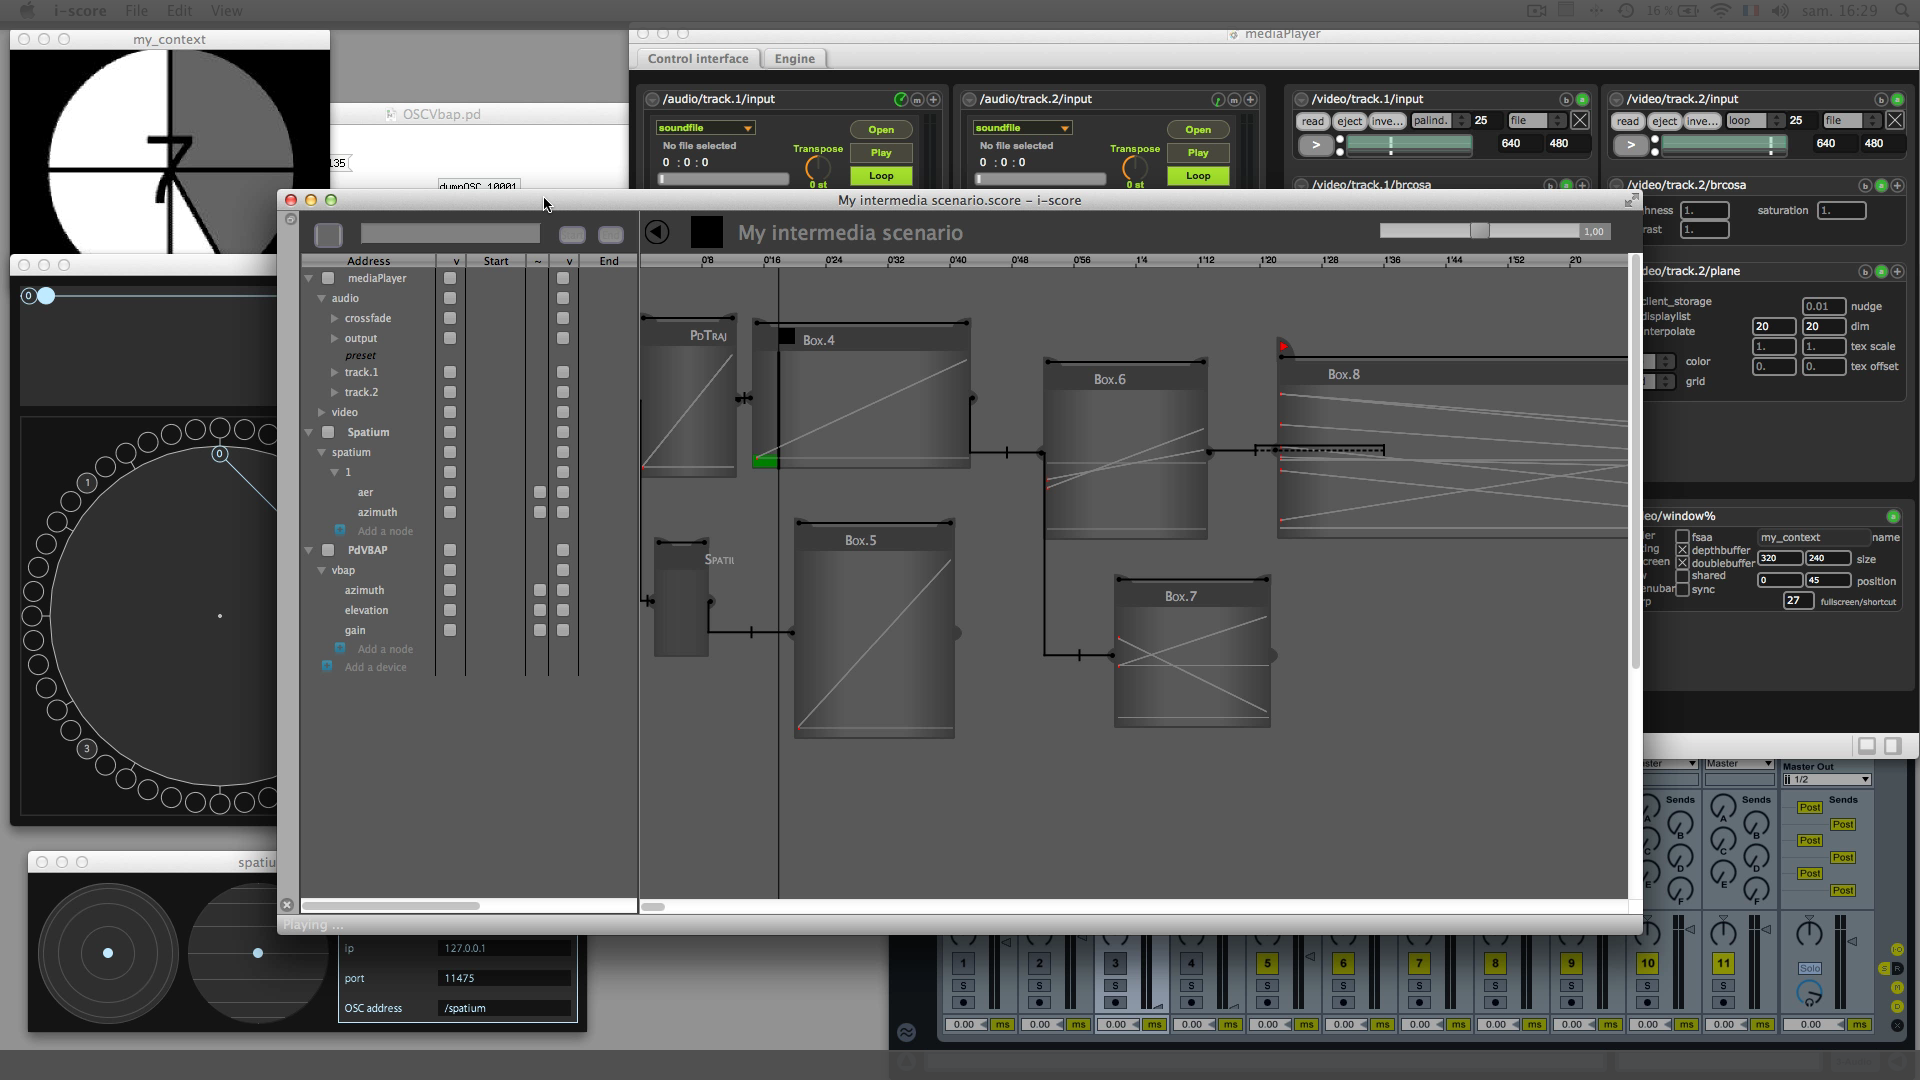
\includegraphics[scale=0.1]{image/iscore.jpg}
\end{center}

I-score est un logiciel qui permet d'avoir sous une seule interface, la possibilité de créer, de synchroniser et d'avoir une interactive de la musique.
\\
C'est un séquenceur basé sur Qt.\\
Qt est une API orienté C++ qui dans notre cas, permet offre des outils de création d'interfaces graphiques.
\paragraph{}
I-score est basé sur le protocole de communication OSC et minuit.
\\
\acrfull{osc} est un protocole de transmission de données entre ordinateurs, robots ou tout autre matériel ou logiciel compatible. Il permet de tout gérer en temps réels. Utilise les protocoles UDP ou TCP pour le réseaux. Il est semblable au format \acrfull{midi} avec de nettes améliorations. Son équivalent minuit permet de faire communiquer un ordinateur avec l'appareil et inversement, contrairement à \acrshort{osc} qui ne peut qu'envoyer des instructions et également utilisé par i-score.
\paragraph{}
L'utilisateur dessine des "boites" dans la partie "scénario" du logiciel. Chaque boites peut correspondre à de la musique, un mouvement d'un robot, de l'éclairage, ..., sur une grille de temps.
\paragraph{}
Chaque boite, peut contenir des fluctuations par des courbes, des droites croissante ou décroissante pour varier une condition au cours du temps.
\\
A chaque tops d'horloge, (c'est à dire lorsque la barre de temps atteint une boite), elle active le paramètre du scénario.

\chapter{Metabot}
\begin{center}
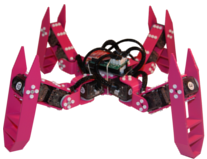
\includegraphics[scale=0.5]{image/metabot.jpg}
\end{center}

\paragraph{}
Le metabot\footnote{http://www.metabot.fr} est un petit robot sous la forme d'araignée disponible à la vente. Ce robot sert essentiellement à apprendre à programmer.
\paragraph{}
Il est composé de 12 moteurs, chacun correspondant à une articulation possible. La structure est faite par impression 3D. 
Il nécessite deux batteries à recharger par usb, une recharge complète prend quelques heures. Nous avons dû nous fournir de quatre batteries par metabot pour pouvoir optimiser la recharge qui prend environ 2h et se fait uniquement par usb.
\paragraph{}
Le metabot peux être commander par instruction simple par un terminal, ou via un logiciel (robotManager) ou par un site internet\footnote{blocks.metabot.fr} qui permet de simuler le comportement du metabot.
\\
Par le terminal, les instructions envoyer modifie directement les paramètres du metabot. Par le site internet ou par le logiciel, les instructions sont envoyé en langage assembleur Rhock, un langage créé pour les besoins du robot.
\paragraph{}
Un  gitHub\footnote{https:// gitHub.com/Rhoban/MetabotManager} est disponible pour le code source du metabot.
\paragraph{}
Le chemin d'accès sur un terminal sous Ubuntu est \texttt{/dev/ttyACM0} pour l'usb, et \texttt{/dev/rfcomm0} pour le bluetooth. 

\paragraph{}
Le site internet permet de compiler directement dans la mémoire du metabot, des instructions (comme par exemple une danse). Il est possible de sauvegarder ces programmes mais pas de le compiler indépendemment du site. Ces fichiers sont sous le format .metablocks, un mélange de xml et d'assembleur Rhock.
\paragraph{}
Les commandes de base pour faire fonctionner sont (x correspond à la variable mise en argument):\\
\begin{itemize}
\item dx x - fait avancer le metabot en avant avec une fréquence de x
\item dy x - fait avancer le metabot de coté avec une fréquence de x
\item crab x - modifie l'angle des 4 pattes de façon symétrique de x degré
\item turn x - fait tourner le metabot sur lui même de x degré
\item start - démarre le metabot (les  leds deviennent verte)
\item stop - arrête le metabot (les  leds deviennent rouge)
\end{itemize}

\section{Connexion pc - metabot}

\paragraph{Ubuntu}
\paragraph{}
Pour manipuler le metabot, on peut passer par un terminal et y rentrer les commandes prédéfinies (pour les connaître il faut lancer la commande params).
\paragraph{}
Pour cela (sous Ubuntu): 
\begin{itemize}
\item cu -l \texttt{/dev/ttyAMC0} (si le metabot est brancher par usb
\item cu -l \texttt{/dev/rfcomm0} (si le metabot est branché par bluetooth
\end{itemize}
\paragraph{}
Concernant le bluetooth, il a fallu désinstaller modemmanager, un gestionnaire des fonctionnalités modem d'Ubuntu, installer de base qui envoyait des instructions aléatoires par bluetooth et installer bluemanager (un gestionnaire sous Ubuntu pour le bluetooth) pour connecté le metabot.

Le metabot doit être connecter avec une clé (1234) qui peut être modifiée et lui allouer un port série.
\paragraph{Windows}
\paragraph{}
Sous Windows, il faut installer robotManager (logiciel fournit sur le site officiel du metabot).

Ce gestionnaire existe sous Ubuntu, mais il doit être lancé par QtCreator et être récupéré par le  gitHub\footnote{https:// gitHub.com/Rhoban/MetabotManager} du metabot.

Le metabot peut se connecter au port série RS-232 (une norme standardisant un bus de communication) correspondant au slot COM0 ou COM1, etc ...

Les commandes sont les plus importantes sont: params,  t, move, freq, \\backLegs, r, h, dx, dy, crab, turn, help, echo, mute, rc, forward, start, stop,\\ dxl\_zero, rhock, run, freeze, kill, killall, erase, erase\_all, meminfo, mem, \\store, version, started.

\section{Modifier le firmware}
\paragraph{}

Si on souhaite installer un firmware modifié il faut le télécharger sur  gitHub\footnote{https:// gitHub.com/Rhoban/Metabot}.
\paragraph{}
Pour le compiler, il faut modifier le Makefile qui se trouve dans le dossier\\ /src/firmware en enlevant les "-Wall" et en rajoutant la ligne suivante \\dans le LDFLAGS:

\texttt{-L./RobotsWars/BinutilsArm/arm-none-eadi/lib/armv6-m/ -lstdc++}.


\paragraph{}
Puis, télécharger les dossiers manquant en faisant ./prepare.sh
\paragraph{}
Si le script n'arrive pas à télécharger les dossiers, il faut faire dans src/ :\\
"mkdir rhock"  \\
Puis ./prepare.sh \\
(ou directement git clone https:// gitHub.com/Rhoban/Rhock).

Après cette étape faire make.

\section{Mettre à jour le metabot}
\paragraph{}
Lors de l'achat d'un metabot, il est fourni avec la première version du firmware (pour vérifier, envoyer la commande "version" au metabot). Pour accéder à toutes les fonctions, il faut donc le mettre à jour.
\paragraph{}
On peux le mettra à jour avec robotManager qui va télécharger la dernière version mise en ligne.
Avec QtCreator sous Ubuntu, on peut modifier l'accès au nouveau firmware en le faisant télécharger une nouvelle version disponible sur l'ordinateur.

Si on souhaite y mettre un firmware personnalisé, il faut compiler le firmware, et :
\begin{itemize}
\item python robotis\_loader.py \texttt{/dev/ttyACM0}
\\ou
\item make install (qui l'envoie uniquement par usb)
\end{itemize}

\section{compiler un programme dans le metabot}
\paragraph{}
Lorsque l'on créer un comportement sous blocks.metabot.fr, on peux le transférer sur le metabot.
\paragraph{}
Pour cela, il faut que le metabot soit au minimum dans la version 1.1.
\paragraph{}
Être connecté sous robotManager, puis passer du simulateur au metabot sous blocks.metabot.fr puis cliquer sur le bouton de compilation du site.
\paragraph{}
Pour lancer ce programme, on peux utiliser l'application mobile (via l'onglet comportement) soit sur le terminal avec "run [id]", id correspond au slot utilisé par le programme, store permettant de connaître sa position. Kill [id] permet de stopper un programme et erase [id] de le supprimer du metabot.
Soit le lancer via l'application mobile sur Android.

\section{Assembleur Rhock}
L'assembleur Rhock est un langage personnalisé pour le metabot.\\
Par exemple, pour appeler la fonction qui gère toues les  leds, il faut d'abord mettre la variable de la fonction dans la pile avec "pushf 4" puis appeler la fonction "call robot\_ leds".
\paragraph{}
Les boucles sont également prisent en compte: repeat\_0 indique la première boucle 0 et repeat\_end\_0 indique où elle s'arrête. Les lignes de codes entre les deux sera répété x fois en fonction du pushf qui a été fait la ligne d'avant.
\paragraph{}
A l'heure actuelle, les fonctions Rhock ne peuvent être appelées par le terminal. Il est obligatoire de passer par la compilation du site internet. Si cette compilation devient indépendante, les scripts écrits pourront faire la liaison entre le terminal et le metabot et à terme de i-score vers le metabot.
\\
Ainsi, on pourra simuler un comportement sur le site internet, le visualiser et l'importer sur i-score pour le synchroniser.
\\
En effet, faire une chorégraphie avec blocks.metabot.fr prend 3 jours entiers pour 1m30 de musique. 
\begin{center}
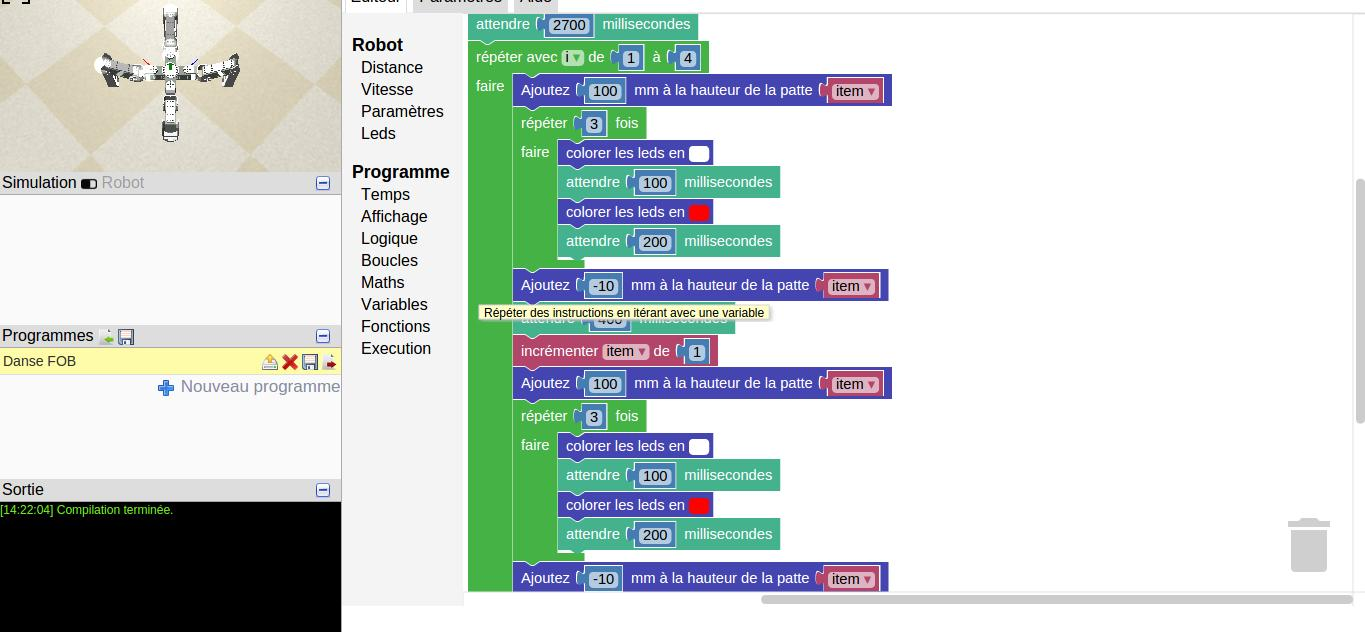
\includegraphics[scale=0.1]{image/site.jpg}
\end{center}
Avec i-score, pour la même durée, cela prend 5h.

\begin{center}
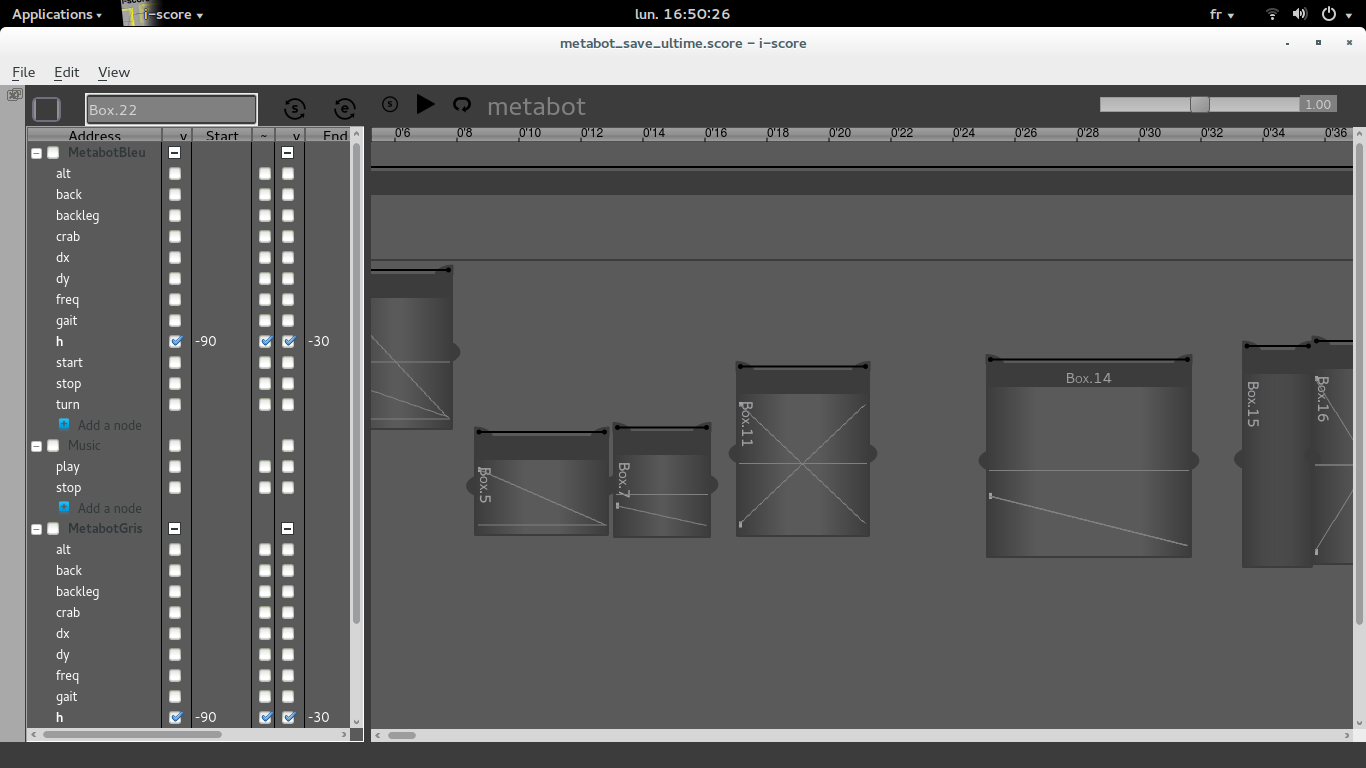
\includegraphics[scale=0.1]{image/danse.png}
\end{center}

\chapter{I-score for metabot}
\section{Les scripts}
\paragraph{}
A partir du site blocks.metabot.fr, nous pouvons récupérer un fichier *.metablocks composé d'une partie xml, et d'une partie assembleur Rhock.
\paragraph{}
Voici un exemple de code *.metablocks qui permet de faire avancer le robot:
\begin{verbatim}
{"id":238,"name":"newProgram","xml":"<xml
xmlns=\"http://www.w3.org/1999/xhtml\">
<block type=\"metabot_move\" id=\"7\"
inline=\"true\" x=\"61\" y=\"43\"><field
name=\"DIR\">FORWARD</field><value
name=\"DIST\"><block type=\"rhock_number\"
id=\"8\"><field    name=\"NUM\">200</field></block>
</value><value name=\"SPEED\"><block 
type=\"rhock_number\" id=\"9\"><field name=\"NUM\">200
</field></block></value></block></xml>",
"code":".thread\nthread_0:\npushf 200
\npushf 200\ncall robot_move_x\n\nstops","vars":[]}
\end{verbatim}
\paragraph{}
N'étant lisible en l'état, il a fallu faire un script pour chaque langage utilisé par ces fichiers. Cela permet de produire un fichier .xml contenant les blocks de commande assembleur sous format "scratch" et un fichier .txt qui comprend uniquement le code assembleur qui sera par la suite modifier pour envoyer des instructions simples au metabot.

\paragraph{}

Ainsi, au lieu d'avoir:
\begin{verbatim} 
pushf 5 
call robot\_ leds
\end{verbatim} 
ce programme écrit en C va prendre le fichier et ligne après ligne envoyé les instructions simple de type : 
\texttt{robot\_ leds 5}
\paragraph{}
Le tout est géré par un script lancement.sh qui permet de ne faire qu'une seule exécution, transforme le tout et l'envoie directement au metabot à partir du fichier .metablocks.

\paragraph{}
\section{La traduction}
\paragraph{}
Pour chaque ligne d'un fichier txt, le programme va chercher des correspondance avec des noms de fonction connus (pushf ou call). Pour chaque pushf, la variable correspondante va être enregistré dans une pile. Dès l'apparition d'un call, la pile est dépiler et on affiche le nom de la fonction correspondante et sa variable sur la même ligne.
\paragraph{}
En cas de fonction de répétition, le programme affiche le contenu de cette boucle autant de fois que le précédent pushf a indiqué.
\paragraph{}
Le résultat final est un fichier test.txt qui comprend toutes les instructions assembleur en instruction simple pouvant être envoyé automatiquement au metabot par le terminal.
\paragraph{}
Tout est généré par un seul script.
\texttt{./lancement <fichier.metablocks>}
\paragraph{}
Ce script s'arrête si on rentre en paramètre un autre format ou si le metabot n'est pas connecté à l'ordinateur.
\paragraph{}
Tout les fichiers produits durant ce stage ou cité dans ce rapport sont open-source et disponible sur  gitHub\footnote{https:// gitHub.com/OSSIA/i-score-metablocks}.

\begin{center}
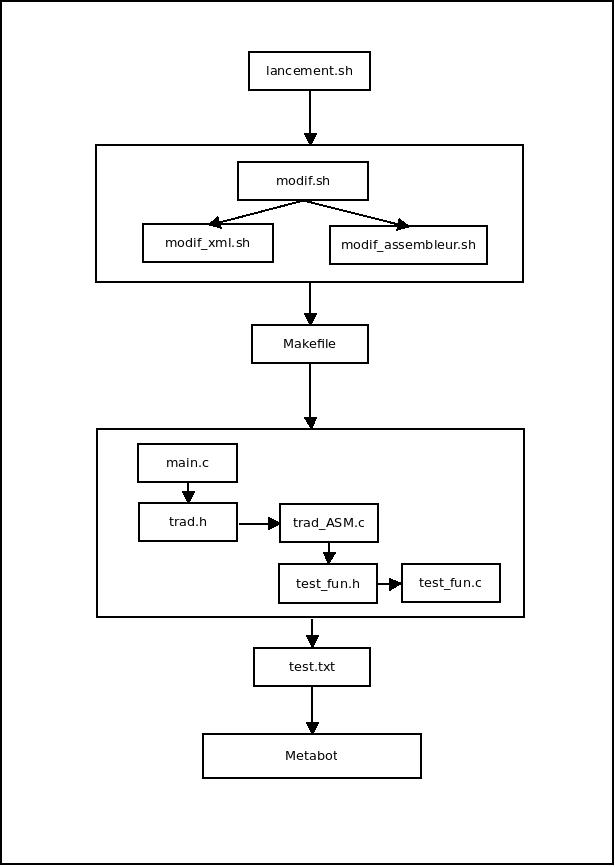
\includegraphics[scale=0.5]{image/schema.jpeg}
\end{center}


\paragraph{}
\chapter{Robot Makers Day}
\paragraph{}
\begin{center}

\includegraphics[scale=0.8]{image/makers.jpg}
\end{center}
\paragraph{}
Le 13 juin s'est déroulé le Robot Makers Day\footnote{http://robotmakersday.fr/}, ce fut l'occasion de montrer notre travail et les perspectives que nous avons.
\paragraph{}
Nous y avons rencontré quelque difficulté. En effet, contrôler un metabot par bluetooth lorsque plusieurs sont présent à cet évènement n'est pas chose aisés. En effet, le nom de l'appareil ne peux être modifier, par conséquent, tous les metabots présents se nommaient robotis-210. Pour pouvoir reconnaître les nôtres, nous regardions la force du signal bluetooth.
\paragraph{}
Ayant eu des problèmes de batterie, de connexion et un temps très limité pour la présentation, nous n'avons malheureusement pas pu montrer tout l'étendu de notre travail.
\paragraph{}
Malgré cela, le public présent fut ravie de notre présentation.

\paragraph{}
\chapter{Perspective}
\paragraph{}
Le stage n'étant que d'un mois, il ne m'a pas été possible de terminer la traduction. En effet, il manque la conversation metabot en fichier de sauvegarde i-score.

Ce fichier de sauvegarde est écrit en \acrfull{json} semblable visuellement à de l'xml.

Il est composé de 4 partie:
\begin{itemize}
\item Constraint qui définit une durée contenant un processus
\item Event permet de mettre des contraintes à la suite les unes des autres
\item Timenode permet de synchroniser des event pour qu'ils s'exécutent en même temps
\item scénario orchestre les contraintes / event / timenodes entre eux
\end{itemize}
et enfin les automations qui correspond aux fluctuation (la courbe) possible à l'intérieur d'un scénario.

Une documentation\footnote{https:// gitHub.com/OSSIA/i-score-metablocks/blob/master/README.md} a été faite pour permettre à la personne qui s'en chargera de mieux comprend le travail effectuer à l'heure actuelle.


\def\appendixpage{\vspace*{8cm} 
\begin{center} 
\Huge\textbf{Annexes} 
\end{center} 
} 
\def\appendixname{Annexe}% 

\begin{appendices} 
\chapter{Documentation} 
\paragraph{}
Contient des scripts pour transformer les fichiers issus du site internet \footnote{http://blocks.metabot.fr/} en fichier assembleur RHOCK et xml qui seront lisible par i-score, un logiciel séquenceur.
\paragraph{}
Pour cela, il faut installer libxml2 : 
\texttt{sudo apt get install libxml2-utils}.
\paragraph{}
Pour lancer et passer de .metablocks à des commandes envoyer au metabot.
\texttt{./lancement.sh fichier.metablocks}
\paragraph{}
Ce dossier contient un fichier \texttt{danse\_FOB.metablocks} qui contient une chorégraphie possible effectuée via le site internet\footnote{blocks.metabot.fr}.
\paragraph{}
Pour la lancer sur le robot, il faut mettre à jour le firmware du metabot vers la \texttt{version 1.1}.
\paragraph{}
Installer robotManager (avec QtCreator sur Ubuntu ou directement via le site metabot.fr) et brancher le metabot par usb à un ordinateur.
\paragraph{}
Pour mettre à jour le metabot:
\begin{itemize}
\item soit être connecté sur robotManager (usb) et mettre à jour le firmware.
\item soit avec un firmware custom dans le dossier.\\
    \texttt{python robotis-loader.py /dev/ttyACM0 metabot.bin}
\item soit ./prepare.sh // make // make install
Pour récupérer le dossier firmware du metabot:
A l'heure actuelle, les fonctions rhocks ne sont pas fournit dans le dossier  gitHub\footnote{git clone https:// gitHub.com/Rhoban/Metabot.git}.
\end{itemize}

\paragraph{}
Il manque donc deux dossiers, pour cela, dans le dossier /firmware/src/ faire ./prepare.sh.
\paragraph{}
Si ce script échoue: dans le dossier /src \texttt{mkdir rhock ./prepare.sh \footnote{ou directement git clone https:// gitHub.com/Rhoban/Rhock}}. \\
Enlever les -Wall du Makefile.\\
Si le Makefile ne trouve pas la bibliothèque libstdc++.a, il faut remplacer la ligne LDFLAGS par  
\texttt{LDFLAGS = $(TARGET_LDFLAGS) $(TOOLCHAIN\_LDFLAGS)\\ 
-mcpu=cortex-m3 -mthumb \ -Xlinker\\ 
--gc-sections \ -Xassembler\\
--march=armv7-m \ \\
-L./RobotsWar/BinutilsArm/arm-none-eabi/lib/armv6-m/ -lstdc++}.
\paragraph{}
Pour compiler une chorégraphie dans le metabot:
- se connecter sur le site blocks.metabot.fr
- importer le fichier danse\_FOB.metablocks
- compiler vers le metabot
Il est possible de lancer cette danse sur un smartphone via l'application Android metabot\footnote{https://play.google.com/store/apps/details?id=fr.metabot.mobile} Ou via un terminal avec run [id].
\paragraph{}
Commande à connaître:
id étant le slot ou ce trouve le programme. Pour le connaître: store.
\paragraph{}
Pour arrêter un programme kill [id] plusieurs kill all. Pour supprimer un programme erase [id] ou erase all.

\chapter{Les scripts} 
\lstinputlisting[caption=lancement.sh, style=custombash]
{i-score-metablocks/lancement.sh}
\newpage
\lstinputlisting[caption=modif.sh, style=custombash]
{i-score-metablocks/script/modif.sh}

\lstinputlisting[caption=modif.sh, style=custombash]
{i-score-metablocks/script/modif_assembleur.sh}

\lstinputlisting[caption=modif.sh, style=custombash]
{i-score-metablocks/script/modif_xml.sh}

\chapter{Les scripts : Résultats} 
\begin{lstlisting}[language=xml, frame=none]
avance.xml

<?xml version="1.0"?>
<block type="metabot_move" 
id="7" inline="true" x="61" y="43">
  <field name="DIR">FORWARD</field>
  <value name="DIST">
    <block type="rhock_number" id="8">
      <field name="NUM">200</field>
    </block>
  </value>
  <value name="SPEED">
    <block type="rhock_number" id="9">
      <field name="NUM">200</field>
    </block>
  </value>
</block>
\end{lstlisting}
\paragraph{}

\begin{verbatim}
avance.txt

.thread
thread_0:
pushf 200
pushf 200
call robot_move_x

stops 
\end{verbatim}
\chapter{La traduction assembleur} 
\lstinputlisting[caption=trad\_ASM.c, style=customc]
{i-score-metablocks/function/trad_ASM.c}

\lstinputlisting[caption=test\_fun.h, style=customc]
{i-score-metablocks/function/test_fun.h}

\lstinputlisting[caption=trad.h, style=customc]
{i-score-metablocks/function/trad.h}
\newpage
\lstinputlisting[caption=test\_fun.c, style=customc]
{i-score-metablocks/function/test_fun.c}

\lstinputlisting[caption=main.c, style=customc]
{i-score-metablocks/function/main.c}

\paragraph{Et son Makefile}
\lstinputlisting[caption=Makefile, style=custombash]
{i-score-metablocks/Makefile}

\chapter{Résultat final envoyé au metabot} 

\lstinputlisting[caption=exemple\_resultat.txt]{i-score-metablocks/exemple_resultat.txt}

\end{appendices} 

\end{document}